%   Filename    : chapter_4.tex 
\chapter{Results and Discussion}
This chapter presents the results on estimating the depth of potholes using the StereoPi system. It details the prototype construction, calibration of the system, and the application of regression analysis to improve depth estimation. It also contains the measurements taken during the testing phases, comparing the ground truth depths with the value estimated by the camera. Findings are presented systematically, supported by tables showing the collected data, images of the outputs, and discussion on the analysis of results.

\section{System Calibration and Model Refinement}
After the initial testing, the system was calibrated using a controlled setup, where artificial potholes with known depths were created. The stereo camera system captured disparity maps, from which depth was calculated using the standard stereo vision formula:

\[
\text{Depth} = \frac{f \times B}{d}
\]

where:
\begin{itemize}
	\item \( f \) is the focal length in pixels,
	\item \( B \) is the baseline distance between the two cameras,
	\item \( d \) is the disparity.
\end{itemize}


However, preliminary observations revealed that the relationship between measured disparity and depth was shifted from the ideal. Their relationship is inherently nonlinear, specifically an inverse relationship (of the form y=1/x). As disparity decreases, depth increases rapidly and nonlinearly. However, due to real-world factors such as lens distortion, imperfect calibration, stereo matching errors, and pixel quantization, the actual relationship between measured disparity and true depth often deviates from the theoretical ideal \cite{scharstein2002}.

To address the shifting behavior, a curve fitting approach was introduced. Specifically, an inverse model was fitted to the collected data points, relating disparity and ground-truth distance measurements.

An inverse function of the form:

\[
y = a + \frac{b}{x}
\]

where:
\begin{itemize}
	\item \( y \) is the estimated distance (in cm),
	\item \( x \) is the measured disparity,
	\item \( a \) and \( b \) are coefficients obtained through regression analysis.
\end{itemize}

%\section{Model Refinement Using Regression}
%The regression analysis produced the following model parameters:
%\begin{itemize}
%	\item a = …
%	\item b = ...
%\end{itemize}

%The model achieved the following performance on the test data:

%\begin{table}[H]
%	\centering
%	\begin{tabular}{|c|c|}
	%		\hline
	%		\textbf{Metric} & \textbf{Value} \\ \hline
	%		Mean Absolute Error (MAE) & X cm \\ \hline
	%		Root Mean Square Error (RMSE) & X cm \\ \hline
	%	\end{tabular}
%	\caption{Performance Metrics for the Regression Model}
%	\label{tab:performance_metrics}
%\end{table}

%The relatively low MAE and RMSE indicate that the fitted model significantly improved the accuracy of depth estimation compared to the original stereo formula.


%\section{Error Analysis}
%Despite the improvements, minor estimation errors remained. These errors were primarily attributed to:
%\begin{itemize}
%	\item Low-light imaging conditions affecting disparity computation,
%	\item Shallow potholes with depths less than 1 cm, where disparity resolution becomes a limiting factor,
%	\item Perspective distortion when the stereo camera was not parallel to the ground plane.
%\end{itemize}


\section{Testing Results}

Following calibration, actual potholes located around the University of the Philippines Visayas (UPV) campus were tested. The ground truth depths of the potholes were measured manually and compared with the depths estimated by the StereoPi camera. Based on the results, the StereoPi camera was able to estimate the depths fairly close to the actual measurements. 

The smallest error occurred in one pothole, where the estimated depth was only 0.02 cm off from the ground truth. The largest observed error was 3.45 cm. Most of the time, the camera’s estimated depths were within approximately 1 to 3 centimeters of the actual depths. This demonstrates reasonable accuracy given the hardware setup and environmental conditions. 

A complete comparison of ground truth and estimated depth values can be found in Appendix C.



\begin{figure}[htbp]
	\centering
	\begin{minipage}{0.32\textwidth}
		\centering
		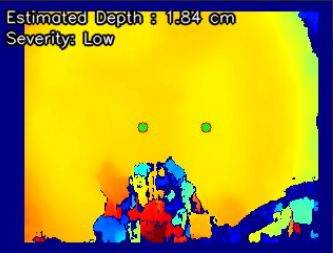
\includegraphics[width=\textwidth]{pothole disparity.png}
		\caption{Disparity Map}
		\label{fig:image1}
	\end{minipage}
	\hfill
	\begin{minipage}{0.32\textwidth}
		\centering
		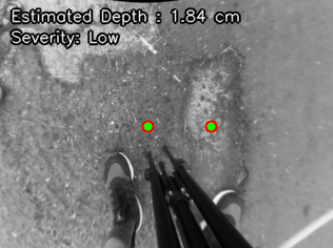
\includegraphics[width=\textwidth]{pothole raw left.png}
		\caption{Left Stereo Image}
		\label{fig:image2}
	\end{minipage}
	\hfill
	\begin{minipage}{0.32\textwidth}
		\centering
		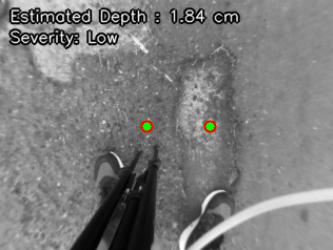
\includegraphics[width=\textwidth]{pothole raw right.png}
		\caption{Right Stereo Image}
		\label{fig:image3}
	\end{minipage}
\end{figure}


The results show that the StereoPi system provides highly accurate estimates of pothole depth. The strong correlation (R=0.978) and high coefficient of determination (R\textsuperscript{2}=0.956) indicate that the actual depth significantly predicts the estimated values. The regression coefficient for actual depth was statistically significant (p $<$ 0.001), suggesting that the relationship is not due to chance. While the RMSE of 0.844 cm and MAE of 0.945 cm suggest generally small errors, the presence of a maximum error of 3.45 cm indicates that there may be occasional outliers or limitations in specific scenarios. Nonetheless, the overall model performance demonstrates that the StereoPi system is suitable for practical pothole depth estimation.

\begin{table}[H]
	\centering
	\begin{tabular}{|c|c|c|c|}
		\hline
		\textbf{R} & \textbf{R\textsuperscript{2}} & \textbf{Root Mean Square Error (cm)} & \textbf{Mean Absolute Error (cm)} \\
		\hline
		0.978 & 0.956 & 0.844 & 0.945 \\
		\hline
	\end{tabular}
	\caption{Linear Regression Model Fit Summary}
	\label{tab:model_fit}
\end{table}

\begin{table}[H]
	\centering
	\begin{tabular}{|l|c|c|c|c|}
		\hline
		\textbf{Predictor} & \textbf{Estimate} & \textbf{SE} & \textbf{t} & \textbf{p} \\
		\hline
		Intercept & 0.159 & 0.2544 & 0.625 & 0.536 \\
		Actual Depth & 0.848 & 0.0317 & 26.752 & \textless 0.001 \\
		\hline
	\end{tabular}
	\caption{Model Coefficients - Estimated Depth}
	\label{tab:model_coefficients}
\end{table}

In figure 4.4, a linear relationship between actual and estimated depth is observed with points closely clustered around the regression line. Indicating the accurate depth estimation. The close alignment of most data points with the fitted line and narrow confidence interval suggest high predictive accuracy and minimal deviation, especially at lower depth values.

\begin{figure}[H]
	\centering
	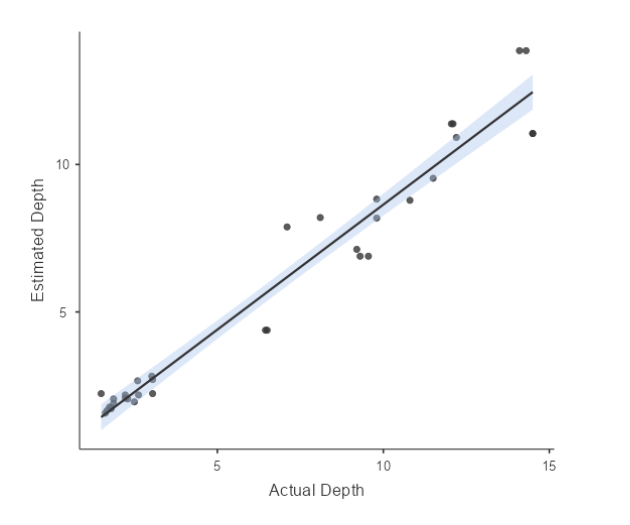
\includegraphics[scale=0.55]{regression.png}
	\caption{Linear Regression Fit Between Actual and Estimated Depth}
	\label{fig:model}
\end{figure}


\section{Discussion}
The study found that stereo vision works effectively in helping estimate the depth of road potholes. The system built using the StereoPi V2 camera was able to measure pothole depths with results mostly within ±3 cm of the actual ground truth values, with an overall root mean square error (RMSE) of 0.844 cm and mean absolute error (MAE) of 0.945 cm. This matches the general observation in earlier studies such as those by Ramaiah and Kundu (2021), which showed that stereo vision can provide useful 3D information for road obstacle detection. However, this study advances previous work by focusing not just on detection, but on depth-based severity classification, which was largely missing in earlier research.

A strong positive correlation (R = 0.978) and coefficient of determination (R\textsuperscript{2} = 0.956) indicate that the actual pothole depths strongly predict the estimated values. The regression model’s significant predictor (p $<$ 0.001) further supports the robustness of the depth estimation approach. This level of accuracy and model performance highlights the suitability of the StereoPi system for practical field applications in pothole monitoring and maintenance prioritization. This finding is significant because earlier machine learning-based road detection studies such as those by Bibi et al. (2021) focused mostly on classifying the existence of defects, not measuring their severity.

The outputs of the system were generally positive, showing that with proper calibration and tuning, consistent and reliable depth estimates can be produced. Calibration using checkerboards and tuning block matching parameters were crucial steps in achieving these results. Similar to the findings of Sanz et al. (2012), proper stereo camera calibration was found to be critical to achieving acceptable disparity maps. This reinforces the importance of calibration techniques, especially in real-world outdoor conditions where environmental factors introduce noise.

However, the study also highlighted limitations affecting system performance, including sensitivity to camera calibration quality, lighting conditions, road surface texture, and the camera's vertical positioning during image capture. Outdoor testing revealed that low lighting and shallow potholes made it difficult to generate clean disparity maps, sometimes causing minor estimation errors. These observations are consistent with Sattar et al. (2018), who reported that mobile road sensing systems often struggle in low-light or highly variable surface conditions. Understanding these challenges is important because it points to practical improvements, such as using better cameras, adding lighting support, or applying more robust image enhancement methods in future versions of the system.
